%%%%%%%%%%%%%%%%%%%%%%%%%%%%%%%%%%%%%%%%%%%%%%%%%%%%%%%%%%%%%%%%%%%%%%
%%  Copyright by Wenliang Du.                                       %%
%%  This work is licensed under the Creative Commons                %%
%%  Attribution-NonCommercial-ShareAlike 4.0 International License. %%
%%  To view a copy of this license, visit                           %%
%%  http://creativecommons.org/licenses/by-nc-sa/4.0/.              %%
%%%%%%%%%%%%%%%%%%%%%%%%%%%%%%%%%%%%%%%%%%%%%%%%%%%%%%%%%%%%%%%%%%%%%%

\newcommand{\commonfolder}{../../common-files}

\documentclass[11pt]{article}

\usepackage[most]{tcolorbox}
\usepackage{times}
\usepackage{epsf}
\usepackage{epsfig}
\usepackage{amsmath, alltt, amssymb, xspace}
\usepackage{wrapfig}
\usepackage{fancyhdr}
\usepackage{url}
\usepackage{verbatim}
\usepackage{fancyvrb}
\usepackage{adjustbox}
\usepackage{listings}
\usepackage{color}
\usepackage{subfigure}
\usepackage{cite}
\usepackage{sidecap}
\usepackage{pifont}
\usepackage{mdframed}
\usepackage{textcomp}
\usepackage{enumitem}


% Horizontal alignment
\topmargin      -0.50in  % distance to headers
\oddsidemargin  0.0in
\evensidemargin 0.0in
\textwidth      6.5in
\textheight     8.9in 

\newcommand{\todo}[1]{
\vspace{0.1in}
\fbox{\parbox{6in}{TODO: #1}}
\vspace{0.1in}
}


\newcommand{\unix}{{\tt Unix}\xspace}
\newcommand{\linux}{{\tt Linux}\xspace}
\newcommand{\minix}{{\tt Minix}\xspace}
\newcommand{\ubuntu}{{\tt Ubuntu}\xspace}
\newcommand{\setuid}{{\tt Set-UID}\xspace}
\newcommand{\openssl} {\texttt{openssl}}


\pagestyle{fancy}
\lhead{\bfseries SEED Labs}
\chead{}
\rhead{\small \thepage}
\lfoot{}
\cfoot{}
\rfoot{}


\definecolor{dkgreen}{rgb}{0,0.6,0}
\definecolor{gray}{rgb}{0.5,0.5,0.5}
\definecolor{mauve}{rgb}{0.58,0,0.82}
\definecolor{lightgray}{gray}{0.90}


\lstset{%
  frame=none,
  language=,
  backgroundcolor=\color{lightgray},
  aboveskip=3mm,
  belowskip=3mm,
  showstringspaces=false,
%  columns=flexible,
  basicstyle={\small\ttfamily},
  numbers=none,
  numberstyle=\tiny\color{gray},
  keywordstyle=\color{blue},
  commentstyle=\color{dkgreen},
  stringstyle=\color{mauve},
  breaklines=true,
  breakatwhitespace=true,
  tabsize=3,
  columns=fullflexible,
  keepspaces=true,
  escapeinside={(*@}{@*)}
}

\newcommand{\newnote}[1]{
\vspace{0.1in}
\noindent
\fbox{\parbox{1.0\textwidth}{\textbf{Note:} #1}}
%\vspace{0.1in}
}


%% Submission
\newcommand{\seedsubmission}{You need to submit a detailed lab report, with screenshots,
to describe what you have done and what you have observed.
You also need to provide explanation
to the observations that are interesting or surprising.
Please also list the important code snippets followed by
explanation. Simply attaching code without any explanation will not
receive credits.}

%% Book
\newcommand{\seedbook}{\textit{Computer \& Internet Security: A Hands-on Approach}, 2nd
Edition, by Wenliang Du. See details at \url{https://www.handsonsecurity.net}.}

%% Videos
\newcommand{\seedisvideo}{\textit{Internet Security: A Hands-on Approach},
by Wenliang Du. See details at \url{https://www.handsonsecurity.net/video.html}.}

\newcommand{\seedcsvideo}{\textit{Computer Security: A Hands-on Approach},
by Wenliang Du. See details at \url{https://www.handsonsecurity.net/video.html}.}

%% Lab Environment
\newcommand{\seedenvironment}{This lab has been tested on our pre-built
Ubuntu 16.04 VM, which can be downloaded from the SEED website. }

\newcommand{\seedenvironmentA}{This lab has been tested on our pre-built
Ubuntu 16.04 VM, which can be downloaded from the SEED website. }

\newcommand{\seedenvironmentB}{This lab has been tested on our pre-built
Ubuntu 20.04 VM, which can be downloaded from the SEED website. }

\newcommand{\seedenvironmentAB}{This lab has been tested on our pre-built
Ubuntu 16.04 and 20.04 VMs, which can be downloaded from the SEED website. }

\newcommand{\nodependency}{Since we use containers to set up the lab environment, 
this lab does not depend too much on our SEED VM. You can do this lab
using other VMs or physical machines. }







\newcommand{\seedlabcopyright}[1]{
\vspace{0.1in}
\fbox{\parbox{6in}{\small Copyright \copyright\ {#1}\ \ by Wenliang Du.\\
      This work is licensed under a Creative Commons
      Attribution-NonCommercial-ShareAlike 4.0 International License.
      If you remix, transform, or build upon the material, 
      this copyright notice must be left intact, or reproduced in a way that is reasonable to
      the medium in which the work is being re-published.}}
\vspace{0.1in}
}






\lhead{\bfseries SEED Labs -- The Mitnick Attack Lab}
\newcommand{\mitnickFigs}{./Figs}

\newcommand{\rsh}{\texttt{rsh}\xspace}

\begin{document}



\begin{center}
{\LARGE The Mitnick Attack Lab}
\end{center}

\seedlabcopyright{2020}


% *******************************************
% SECTION
% ******************************************* 
\section{Overview}

Kevin Mitnick is probably one of the most well-known hackers in USA. 
He was on FBI's wanted list of criminals. While on the run, 
he became interested in hacking cellular phone networks, and was in need for 
specialized software that could help him do that. 
That led him to Tsutomu Shimomura, a researcher working at 
the San Diego Supercomputer Center, who was
one of the leading researchers on the security of cellular phone networks.
He had the code that Mitnick wanted.

In 1994, Mitnick successfully launched an attack on Shimomura's computer,
by exploiting the vulnerabilities in the TCP protocol
and the trusted relationship between 
two of Shimomura's computers. The attack
triggered a dramatic showdown between the two people, and
it eventually led to the arrest of Mitnick. The showdown 
was turned into books and Hollywood movies later. 
The attack is now known as the Mitnick attack, which is a special type of
TCP session hijacking.


The objective of this lab is to recreate the classic Mitnick attack, 
so students can gain the first-hand experience on such an attack. 
We will emulate the settings that was originally on 
Shimomura's computers, and then 
launch the Mitnick attack to create a forged TCP session between
two of Shimomura's computers. If the attack is successful, 
we should be able to run any command on Shimomura's computer. 
This lab covers the following topics:

\begin{itemize}[noitemsep]
\item TCP session hijacking attack
\item TCP three-way handshake protocol
\item The Mitnick attack
\item Remote shell \rsh
\item Packet sniffing and spoofing
\end{itemize}


\paragraph{Readings and videos.}
Detailed coverage of the TCP session hijacking can be found in the following:

\begin{itemize}
\item Chapter 16 of the SEED Book, \seedbook
\item Section 6 of the SEED Lecture, \seedisvideo
\end{itemize}

\paragraph{Lab environment.} \seedenvironmentB



% *******************************************
% SECTION
% ******************************************* 
\section{How the Mitnick Attack Works}

The Mitnick attack is a special case of TCP session hijacking attacks. 
Instead of hijacking an existing TCP connection between victims A and B, 
the Mitnick attack creates a TCP connection between A and B first on 
their behalf, and then naturally hijacks the connection.  


In the actual Mitnick attack, host A was called X-Terminal, 
which was the target. Mitnick
wanted to log into X-Terminal and run his commands on it. 
Host B was a trusted server, which was allowed to log into X-Terminal without a password.  
In order to log into X-Terminal, Mitnick had to impersonate the trusted server, so
he did not need to provide any password. Figure~\ref{tcp:mitnick} depicts
the high-level picture of the attack. 
There are four primary steps in this attack.


\begin{figure}[htb]
\centering
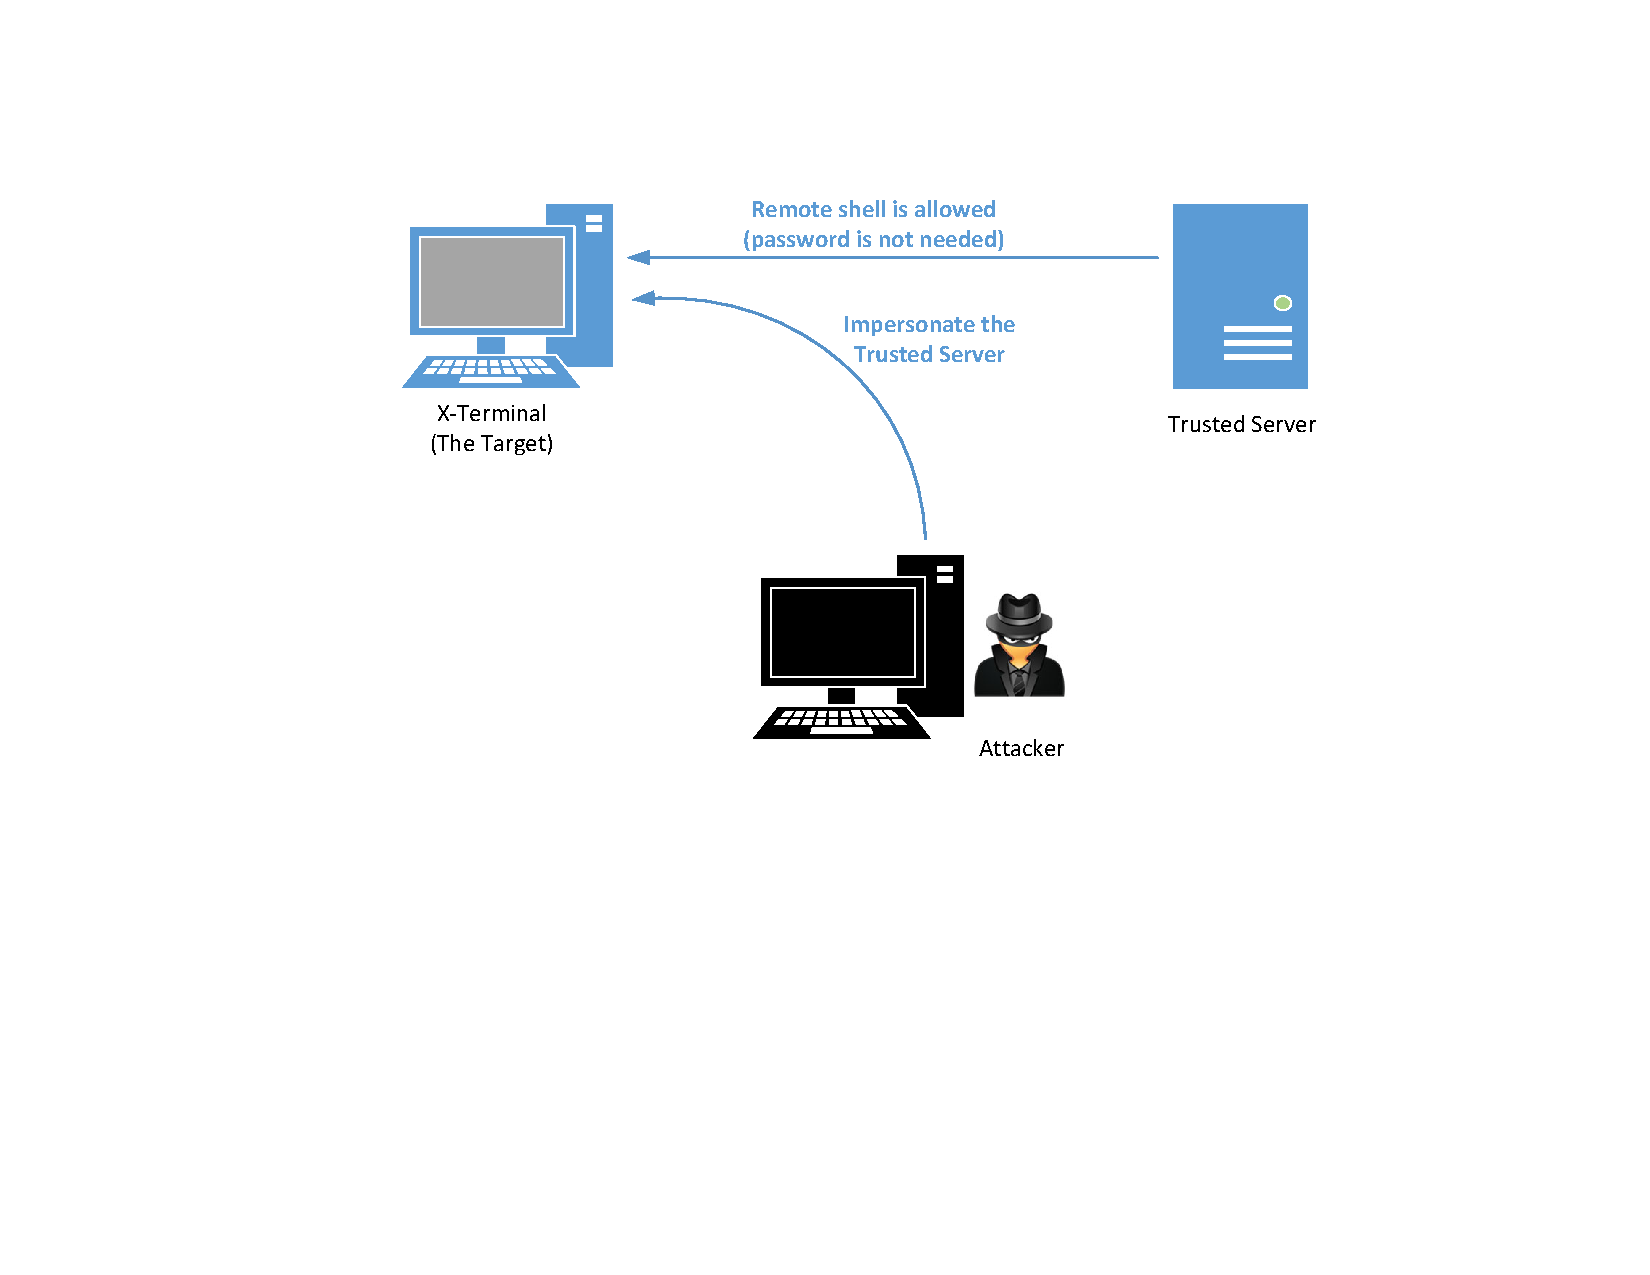
\includegraphics[width=0.8\textwidth]{\mitnickFigs/mitnick_attack.pdf}
\caption{The illustration of the Mitnick Attack}
\label{tcp:mitnick}
\end{figure}


\paragraph{Step 1: Sequence number prediction.} 
Before the attack, Mitnick needed to learn the pattern of the initial sequence numbers (ISN)
on X-terminal (in those days, ISNs were not random). 
Mitnick sent SYN requests to X-terminal and received SYN+ACK responses, 
then he sent
RESET packet to X-Terminal, to clear the half-open connection
from X-Terminal's queue (to prevent the queue from being filled up). After repeating
this for twenty times. He found there was a pattern between two successive
TCP ISNs. This allowed Mitnick to predict ISNs, which was essential for
the attack. 


\paragraph{Step 2: SYN flooding attack on the trusted server.} To
send a connection request from the trusted server to X-Terminal,
Mitnick needed to send out a SYN packet from
the trusted server to X-Terminal. X-Terminal would respond with a
SYN+ACK packet, which was sent to the trusted server. Since the trusted server
did not actually initiate the request, it would send a RESET packet 
to X-Terminal, asking X-Terminal to stop the 3-way handshake. This behavior
caused trouble to the Mitnick attack.

To solve this problem. Mitnick had to silence the trusted server. 
Therefore, before spoofing, Mitnick launched a SYN
flooding attack on the server. Back then, operating systems were far more
vulnerable to the SYN flooding attack.  The attack could actually shut down the
trusted computer, completely silencing it. 


\paragraph{Step 3: Spoofing a TCP connection.} Mitnick wanted to 
use \rsh (remote shell) to run a backdoor command on X-Terminal; once the 
backdoor was setup, he could then log into X-Terminal. 
To run a remote shell on X-Terminal, Mitnick needed to pass the 
authentication, i.e, he needed to have a valid account on X-Terminal and know
its password. Obviously, he did not have that.

Shimomura often needed to log into X-Terminal from the trusted server. To 
avoid typing passwords each time, he added some information
in the \texttt{.rhosts} file on X-Terminal, so when he logged into
X-Terminal from the trusted server, no password would be asked. This was quite a 
common practice back then. With this setup,
without typing any password, 
Shimomura could run a command on X-Terminal from the trusted server using 
\rsh, or run \texttt{rlogin} to log into X-Terminal. 
Mitnick wanted to exploit this trusted relationship.


He needed to create a TCP connection between the trusted server and
X-Terminal, and then run \rsh inside this connection.   
He first sent a SYN request to X-Terminal, using the trusted server's IP as the source IP address.
X-Terminal then sent a SYN+ACK response to the server. Since the server had been shut
down, it would not send RESET to close the connection. 

To complete the three-way handshake protocol, Mitnick needed to spoof
an ACK packet, which must acknowledge the sequence number in 
X-Terminal's SYN+ACK packet. Unfortunately, 
the SYN+ACK response only went to the trusted server, not to Mitnick,
he could not see the sequence number. However, 
because of the prior investigation, Mitnick was able to
predict what this number was, so he was able to 
successfully spoof the ACK response sent to X-Terminal to complete the TCP three-way
handshake. 


\paragraph{Step 4: Running a remote shell.} 
Using the established TCP connection between the trusted server and X-Terminal, Mitnick
could send a remote shell request to X-terminal, asking 
it to run a command. Using this command, 
Mitnick wanted to create a
backdoor on X-Terminal so that he could get a shell 
on X-Terminal anytime without repeating the attack. 

All he needed to do was to add  
\texttt{"+ +"} to the \texttt{.rhosts} file on X-Terminal.
He could achieve that
by executing the following command using \rsh on X-Terminal: 
{\tt "echo + + > .rhosts"}. 
Since \rsh and \texttt{rlogin} program used
\texttt{.rhosts} file for authentication, with this addition, 
X-Terminal would trust every
\rsh and \texttt{rlogin} request from anyone. 



% *******************************************
% SECTION
% ******************************************* 
\section{Lab Environment Setup Using Container}



% -------------------------------------------
% SUBSECTION
% ------------------------------------------- 
\subsection{Container Setup}

In this lab, students need to use three machines, 
one for X-Terminal, one for Trusted Server, and the other for the attacker. 
In the real Mitnick attack, the attacker machine is a remote machine. 
In this lab, for the 
sake of simplicity, we put all these three machines on the same network. 
Students can use three virtual
machines for this lab, but it will be much more convenient to
use one VM plus two containers.  We will launch
attacks from the VM, while using containers for the attack targets. 
We have named the containers using X-Terminal and Trusted Server.
The lab environment is depicted in the following:


\begin{lstlisting}[backgroundcolor=]
            +------------+      +--------------+  +----------------+  
            |     VM     |      |   Container  |  |    Container   |  
            | (attacker) |      | (X-Terminal) |  |(Trusted Server)|  
            |  10.9.0.1  |      |   10.9.0.5   |  |    10.9.0.6    |  
            +----+-------+      +-------+------+  +--------+-------+  
                 | br-<id>             | eth0          | eth0   
                 |                     |               |        
           ------+---------------------+---------------+--------------
           Network  10.9.0.0/24

\end{lstlisting}


%%%%%%%%%%%%%%%%%%%%%%%%%%%%%%%%%%%%%%%%%%%%
% Input common files related to containers

\paragraph{Container setup and commands.}



The Docker and Compose files, along with the user manual,
can be downloaded from the lab's website,
The followings Compose commands are for creating and tearing down
the lab environment. 
Since we are going to use 
these commands and several docker commands very
frequently, we have created aliases for these commands
in the \texttt{.bashrc} file.  


\begin{lstlisting}
$ docker-compose build  # Build the container image
$ docker-compose up     # Start the container
$ docker-compose down   # Shut down the container

// Aliases for commonly used docker and Compose commands. 
$ dcbuild       # Alias for: docker-compose build
$ dcup          # Alias for: docker-compose up
$ dcdown        # Alias for: docker-compose down
$ dockps        # Alias for: docker ps --format "{{.ID}}  {{.Names}}" 
$ docksh <id>   # Alias for: docker exec -it <id> /bin/bash
\end{lstlisting}



Detailed explanation of \texttt{Dockerfile} and
the \texttt{docker-compose.yml} file can be found from
the manual, which is linked to this lab's website. If you encounter
issues when setting up the lab environment, read the
``Common Problems'' section for potential solutions.



\paragraph{Getting the network interface name.}
When we use the provided Compose file to create
containers for this lab, a new network is created
to connect the VM and the containers. The
IP prefix for this network is \texttt{10.9.0.0/24},
which is specified in the \texttt{docker-compose.yml}
file. The IP address assigned to our VM is
\texttt{10.9.0.1}. We need to find the name of
the corresponding network interface on our VM, because we
need to use it in our programs.
The interface name is the concatenation of \texttt{br-}
and the ID of the network created by Docker.
When we use \texttt{ifconfig} to list network interfaces,
we will see quite a few. Look for the IP address
\texttt{10.9.0.1}.


\begin{lstlisting}
$ ifconfig
(*@\textbf{br-c93733e9f913}@*): flags=4163<UP,BROADCAST,RUNNING,MULTICAST>  mtu 1500
        inet (*@\textbf{10.9.0.1}@*)  netmask 255.255.255.0  broadcast 10.9.0.255
        ...
\end{lstlisting}


Another way to get the interface name is to use the \texttt{"docker network"} command to
find out the network ID ourselves (the name of the network is \texttt{seed-net}:

\begin{lstlisting}
$ docker network ls
NETWORK ID          NAME                DRIVER              SCOPE
a82477ae4e6b        bridge              bridge              local
e99b370eb525        host                host                local
df62c6635eae        none                null                local
(*@\textbf{c93733e9f913}@*)        seed-net            bridge              local
\end{lstlisting}



%%%%%%%%%%%%%%%%%%%%%%%%%%%%%%%%%%%%%%%%%%%%





% -------------------------------------------
% SUBSECTION
% ------------------------------------------- 
\subsection{Installing the \rsh program}

The remote shell \rsh is a command line program that can execute shell commands
remotely. Although we will use \rsh in this task, we should know that 
\rsh and \texttt{rlogin} programs are not secure, and they 
are not used any more. They have been replaced by
more secured programs, such as \texttt{ssh}.   
That is why in the modern Linux operating systems, the \rsh command 
is actually a symbolic link to the \texttt{ssh} program. 

\begin{lstlisting}
$ ls -al /etc/alternatives | grep rsh
lrwxrwxrwx   1 root root    12 Jul 25  2017 rsh -> /usr/bin/ssh
\end{lstlisting}



To recreate the Mitnick attack, we need to install the unsecure version
of the \rsh program. Obviously, the old version of 
the \rsh no longer works, but an open-source project
re-implements the remote shell clients and servers. 
It is called \texttt{rsh-redone}. 
We can use the following commands to install \rsh server and client. 

\begin{lstlisting}
$ sudo apt-get install rsh-redone-client
$ sudo apt-get install rsh-redone-server
\end{lstlisting}

\paragraph{Note.} The \rsh programs are already installed in our 
VM and container. 



% -------------------------------------------
% SUBSECTION
% ------------------------------------------- 
\subsection{Configuration}
\label{subsec:configuration}

The \rsh server program uses two files for authentication, 
\texttt{.rhosts} and \texttt{/etc/hosts.equiv}.
Every time the server receives a remote command request, it will check
the \texttt{/etc/hosts.equiv}. If the request comes from a hostname stored in the file, the
server will accept it without asking for passwords. 
If \texttt{/etc/hosts.equiv} does not exist or
do not have that hostname, \rsh  will check the \texttt{.rhosts} file 
on the user's home directory. 

Shimomura often needed to run remote commands on X-Terminal
from the trusted server. To avoid typing passwords, he
created a \texttt{.rhosts} file on host X-Terminal and put the trusted
server's IP address into the file.
Note that the \texttt{.rhosts} file must reside at the top level of a user's home directory and
can be written \textbf{only by the owner/user}.


Please use the following commands on X-Terminal to set up the \texttt{.rhosts} file.
It should be noted when we get into a container, we will be in the root 
account. In this lab, we need to switch to a normal user account called seed, which
is already created inside the container: 

\begin{lstlisting}
# su seed          (*@\reflectbox{\ding{217}}@*) Switch to the seed account
$ cd               (*@\reflectbox{\ding{217}}@*) Go to seed's home directory
$ touch .rhosts    (*@\reflectbox{\ding{217}}@*) Create an empty file 
$ echo [Server's IP address] > .rhosts
$ chmod 644 .rhosts
\end{lstlisting}

To verify your configuration, try running the following command on the trusted server.
\begin{lstlisting}
# su seed          (*@\reflectbox{\ding{217}}@*) Switch to the seed account
$ rsh [X-Terminal's IP] date
\end{lstlisting}

If the command prints the current date and time, your configuration is working now. If you
see ``Authentication Failure'', something in your setup may not be correct. 
One of the common mistakes is the permission on the \texttt{.rhosts} file:
you should make sure it is only writable to the owner.


\paragraph{Allow all.} To allow users to execute commands on X-Terminal from 
all IP addresses, we just need to put two plus signs (\texttt{"+ +"})
in the \texttt{.rhosts} file. This is very dangerous, and nobody should 
do that. But if you are an attacker, this is a convenient way
to set up a backdoor. As we have mentioned before, this is what has been used in
the Mitnick attack. 



% *******************************************
% SECTION
% ******************************************* 
\section{Task 1: Simulated SYN flooding}

The operating systems at the time of the Mitnick Attack were vulnerable to SYN
flooding attacks, which could mute the target machine or even shut it down. 
However, SYN flooding can no longer cause such a damage for modern operating systems. 
We will simulate this effect. 

We can manually stop the trusted server container, but that is not enough.
When X-Terminal receives a SYN packet from the trusted server, it will respond with
a SYN+ACK packet. Before sending out this packet, 
it needs to know the MAC address of the trusted server. 
The ARP cache will be checked first. If there is no entry
for the trusted server, X-Terminal will send out an ARP request packet 
to ask for the MAC address. Since the trusted server has been
muted, no one is going to answer the ARP request, hence 
X-Terminal cannot send out the response. As a result, the
TCP connection will not be established. 

In the real attack, the trusted server's MAC address was actually in X-Terminal's ARP
cache. Even if it was not, before silencing the trusted server, 
we could simply spoof an ICMP echo request from the trusted 
server to X-Terminal, that would trigger X-Terminal to reply to 
the trusted server, and hence would get the trusted server's MAC address, and 
save it to the cache. 


To simplify the task, before stopping the trusted server, 
we will simply ping it from X-Terminal once, and then use 
the \texttt{arp} command to check and make sure that
the MAC address is in the cache. It should be noted that 
cache entry may be deleted by the operating system if 
the OS fails to reach a destination using 
the cached MAC address. To simply your attack, 
you can run the following command on X-Terminal to
permanently add an entry to the ARP cache (it needs to
run in the root account):

\begin{lstlisting}
# arp -s [Server's IP] [Server's MAC]
\end{lstlisting}



% *******************************************
% SECTION
% ******************************************* 
\section{Task 2: Spoof TCP Connections and \rsh Sessions}
\label{sec:task2}

Now that we have ``brought down'' the trusted server, we can impersonate the trusted
server, and try to launch a \rsh session  
with X-Terminal. Since \rsh runs on top of TCP, we first need to 
establish a TCP connection between the trusted server and X-Terminal,
and then run the \rsh in this TCP connection.  


One of the difficulties in the Mitnick attack is to predict the TCP sequence numbers. 
It was possible back then when TCP sequence numbers were not randomized. 
However, modern operating systems now randomize their TCP sequence numbers
(as a countermeasure against TCP session hijacking attacks), so
predicting the numbers becomes infeasible.
To simulate the situation of the original Mitnick attack, we 
allow students to sniff packets, so
they can get the sequence numbers, instead of guessing them.  

\paragraph{Restriction.} To simulate the original Mitnick attack
as closely as we can, even though students can sniff
the TCP packets from X-Terminal, they cannot use all the 
fields in captured packets, because in the real attacks,
Mitnick could not sniff packets. When students write their 
attack programs, they can only use the 
following fields from the captured packets. Penalty will be 
applied if other fields are used.

\begin{itemize}
\item \textbf{The TCP sequence number field} (this does not include the acknowledgment
field).

\item \textbf{The TCP flag field}. This allows us to know the types of the 
captured TCP packets. In the actual Mitnick attack, Mitnick knew
exactly what type of packets were sent out by X-Terminal, because 
they are part of the TCP three-way handshake protocol. 
We allow students to use this field for task simplification. 


\item \textbf{All the length fields}, including IP header length, IP total length,
and TCP header length. These pieces of information are not necessary 
for the attacks. In the actual Mitnick attack, Mitnick knew exactly what their
values are. We allow students to use these fields for task simplification. 
\end{itemize}


\paragraph{The behavior of \rsh.} 
To create a spoofed \rsh session between the trusted server and X-Terminal,
we need to understand the behavior of \rsh. Let us start a 
\rsh session from Trusted Server to X-Terminal, and then use Wireshark
to capture the packets between them (note: we will run Wireshark
on the attacker VM; make sure to select the correct network
interface corresponding to the \texttt{10.9.0.0/24} network). 
We use the following command to
run the \texttt{date} command on Host B from Host A via the \rsh  
remote shell.


\begin{lstlisting}
// On Trusted Server
$ rsh 10.9.0.5 date
\end{lstlisting}
 
The packet trace in this \rsh session is shown in the following. 
Here \texttt{10.9.0.6} is the Trusted Server's IP address, 
and \texttt{10.9.0.5} is X-Terminal's IP address.
If a packet does not carry any TCP data, the length information (i.e.
\texttt{Len=0}) is omitted. 

\begin{lstlisting}[caption={Packet trace of a \rsh session},
                  label={listing:rsh}]
# The first connection
   SRC IP    DEST IP   TCP Header
1  10.9.0.6  10.9.0.5  1023 -> 514 [SYN] Seq=778933536 
2  10.9.0.5  10.9.0.6  514 -> 1023 [SYN,ACK] Seq=10879102 Ack=778933537 
3  10.9.0.6  10.9.0.5  1023 -> 514 [ACK] Seq=778933537 Ack=10879103 
4  10.9.0.6  10.9.0.5  1023 -> 514 [ACK] Seq=778933537 Ack=10879103 Len=20
                       RSH Session Establishment
                       Data: 1022\x00seed\x00seed\x00date\x00
5  10.9.0.5  10.9.0.6  514 -> 1023 [ACK] Seq=10879103 Ack=778933557

# The second connection
6  10.9.0.5  10.9.0.6  1023 -> 1022 [SYN] Seq=3920611526 
7  10.9.0.6  10.9.0.5  1022 -> 1023 [SYN,ACK] Seq=3958269143 Ack=3920611527 
8  10.9.0.5  10.9.0.6  1023 -> 1022 [ACK] Seq=3920611527 Ack=3958269144 


# Going back to the first connection
9  10.9.0.5  10.9.0.6  514 -> 1023 [ACK] Seq=10879103 Ack=778933557 Len=1
                       Data: \x00
10 10.9.0.6  10.9.0.5  1023 -> 514 [ACK] Seq=778933557 Ack=10879104 
11 10.9.0.5  10.9.0.6  514 -> 1023 [ACK] Seq=10879104 Ack=778933557 Len=29
                       Data: Sun Feb 16 13:41:17 EST 2020
\end{lstlisting}


We can observe that a \rsh session consists of two TCP connections.  
The first connection is initiated by Host A (the client). 
An \texttt{rshd} process on Host B is listening to connection requests at port 514. 
Packets 1 to 3 are for the three-way handshake protocol. 
After the connection has been established, the client 
send \rsh data (including user IDs and commands) to the Host B (Packet 4).
The \texttt{rshd} process will authenticate the user, and 
if the user is authenticated, \texttt{rshd} initiates a
separate TCP connection with the client. 


The second connection is used for sending error messages. 
In the trace above, since there was no error, the connection was never used, 
but the connection must be successfully established, or \texttt{rshd} 
will not continue. Packets 6 to 7 are for the three-way handshake protocol
of the second connection. 


After the second connection has been established, 
Host B will send a zero byte to the client (using the first connection),
Host A will acknowledge the packet. After that, \texttt{rshd} on Host B
will run the command sent by the client, and the
output of the command will be sent back to the client, all via the 
first connection. 
Students can use Wireshark to capture a \rsh session, and study its
behaviors, before launching the Mitnick attack. 
We divide the attack task into two sub-tasks, each one focusing on one connection. 



% -------------------------------------------
% SUBSECTION
% ------------------------------------------- 
\subsection{Task 2.1: Spoof the First TCP Connection}
\label{sec:first-conn}

The first TCP connection is initiated by the attacker via a spoofed SYN packet. As you can see
in Figure~\ref{fig:first-conn}, after X-Terminal receives the SYN packet, it will in turn send
a SYN+ACK packet to the trusted server. Since the server has been brought down, it will not
reset the connection. The attacker, which is on the same network, can sniff the packet and get
the sequence number.

\begin{figure}[htb]
\centering
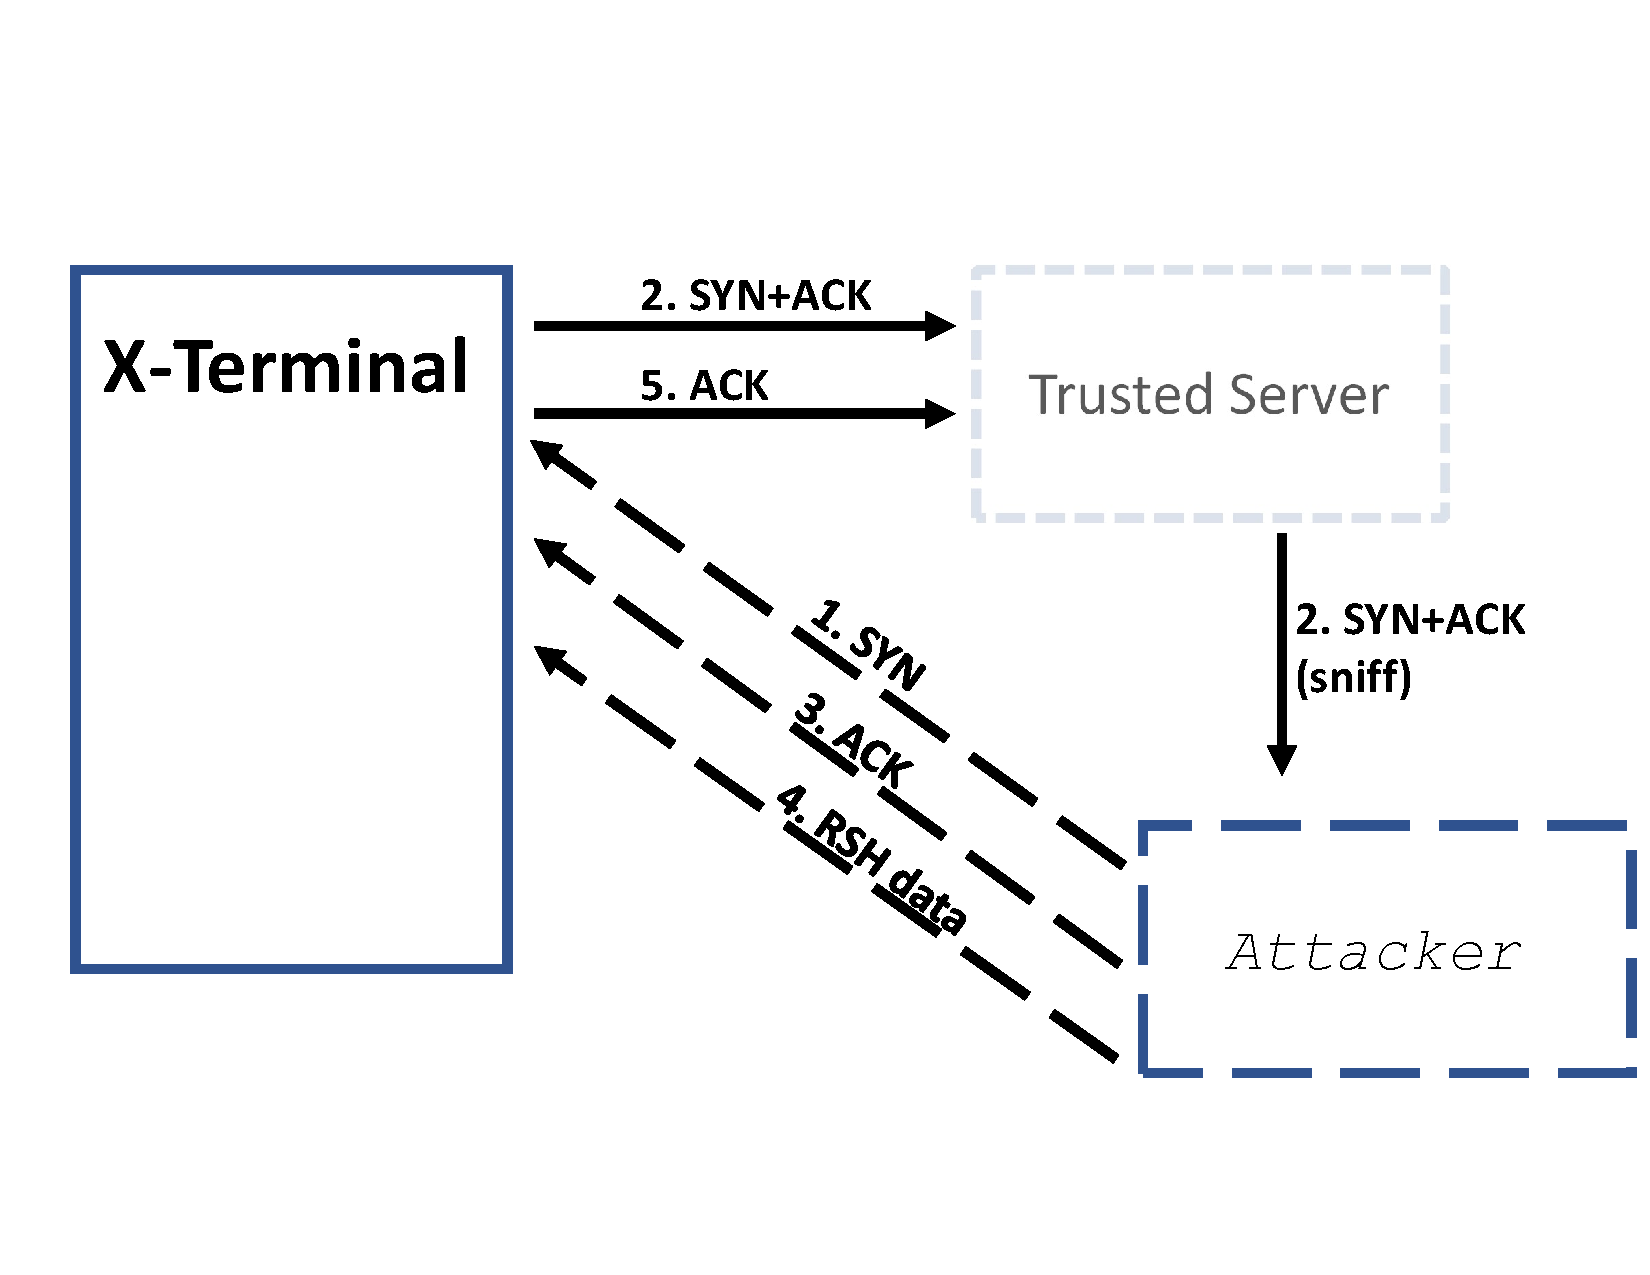
\includegraphics[width=0.6\textwidth]{\mitnickFigs/mitnick-diagram-1.pdf}
\caption{First Connection}
\label{fig:first-conn}
\end{figure}


\paragraph{Step 1: Spoof a SYN packet.}
Students should write a program to spoof a SYN packet 
from the trusted server to X-Terminal (see Packet 1 in Listing~\ref{listing:rsh}). 
There are six standard 
TCP code bits, and they can be set in the flag field of the TCP header. 
The following code examples show how to set the flag field
and how to check whether certain bits are set in
the flag field. 

\begin{lstlisting}
# 'U': URG bit
# 'A': ACK bit
# 'P': PSH bit
# 'R': RST bit
# 'S': SYN bit
# 'F': FIN bit

tcp = TCP()

# Set the SYN and ACK bits
tcp.flags = "SA"

# Check whether the SYN and ACK are the only bits set
if tcp.flags == "SA": 

# Check whether the SYN and ACK bits are set
if 'S' in tcp.flags and 'A' in tcp.flags: 
\end{lstlisting}

It should be noted that the source port of the SYN packet 
must be from port \texttt{1023}. If a different port 
is used, \rsh will reset the connection 
after the connection is established.  If this step is successful, 
from Wireshark, we should be
able to see a SYN+ACK packet coming out of 
X-Terminal (see Packet 2 in Listing~\ref{listing:rsh}).


\paragraph{Step 2: Respond to the SYN+ACK packet.}
After X-Terminal sends out a SYN+ACK, the trusted server needs 
to send out an ACK packet to complete the three-way handshake protocol. 
The acknowledge number in the packet should be \texttt{S+1}, where 
\texttt{S} is the sequence number contained in the SYN+ACK packet. 
See Packet 3 in Listing~\ref{listing:rsh}.

In the actual Mitnick attack, the attacker could not see the SYN+ACK packet, because
it was sent to the trusted server, not to the attacker. 
That is why Mitnick had to guess the value of the sequence number.
In this lab, we allow students to get 
the sequence number via packet sniffing. 

Students need to write a sniff-and-spoof program using \texttt{Scapy} and run it
on the attacker's machine. Here is a skeleton of a sniff-and-spoof program that might be
useful. Please make sure to follow the restrictions described at the
beginning of the section, or you will get a penalty. 


\begin{lstlisting}
#!/usr/bin/python3
from scapy.all import *

x_ip      = "10.9.0.5"  # X-Terminal
x_port    = 514         # Port number used by X-Terminal

srv_ip    = "10.9.0.6"  # The trusted server
srv_port  = 1023        # Port number used by the trusted server

# Add 1 to the sequence number used in the spoofed SYN
seq_num     = 0x1000 + 1


def spoof(pkt):
  global seq_num   # We will update this global variable in the function

  old_ip  = pkt[IP]
  old_tcp = pkt[TCP]

  # Print out debugging information
  tcp_len = old_ip.len - old_ip.ihl*4 - old_tcp.dataofs*4  # TCP data length
  print("{}:{} -> {}:{}  Flags={} Len={}".format(old_ip.src, old_tcp.sport,
                         old_ip.dst, old_tcp.dport, old_tcp.flags, tcp_len))



  # Construct the IP header of the response
  ip = IP(src=srv_ip, dst=x_ip)

  # Check whether it is a SYN+ACK packet or not;
  #   if it is, spoof an ACK packet

  # ... Add code here ...

myFilter = 'tcp'   # You need to make the filter more specific
sniff(iface='br-****', filter=myFilter, prn=spoof)
                  (*@\reflectbox{\ding{218}} \textbf{You need to set the correct value here.}@*)   
\end{lstlisting}




\paragraph{Step 3: Spoof the \rsh data packet.}
Once the connection is established, the attacker needs to 
send \rsh data to X-Terminal.
The structure of the \rsh data is shown below.

\begin{lstlisting}
[port number]\x00[uid_client]\x00[uid_server]\x00[your command]\x00
\end{lstlisting}

The data has four parts: a port number, client's user ID, server's user ID,
and a command.
The port number will be used for the second connection (see Task 2.2). 
Both client and server's user ID is \texttt{seed} in our container. 
The four fields are separated by a byte 0.
Note that there is also a byte 0 at the end of the \rsh data. An example is given in the
following. In this example, we tell X-Terminal that we are going to listen on port 9090 for the
second connection and the command we want to run is \texttt{"touch /tmp/xyz"}. 

\begin{lstlisting}
data = '9090\x00seed\x00seed\x00touch /tmp/xyz\x00'
send(IP()/TCP()/data, verbose=0)
\end{lstlisting}
 

Students should modify the sniff-and-spoof program written in Step 2, so
an \rsh data packet is sent to X-Terminal (see Packet 4 
in Listing~\ref{listing:rsh}). 
If this step is successful, from Wireshark, we can see
that X-Terminal is going to initiate a TCP connection to the trusted server's port
\texttt{9090}, which is the port number specified in our \rsh data.  

In your report, please describe whether the \texttt{touch} command 
has been executed on X-Terminal or not. Please also 
include snapshots of your Wireshark. 


% -------------------------------------------
% SUBSECTION
% ------------------------------------------- 
\subsection{Task 2.2: Spoof the Second TCP Connection}
\label{sec:second-conn}

\begin{figure}[htb]
\centering
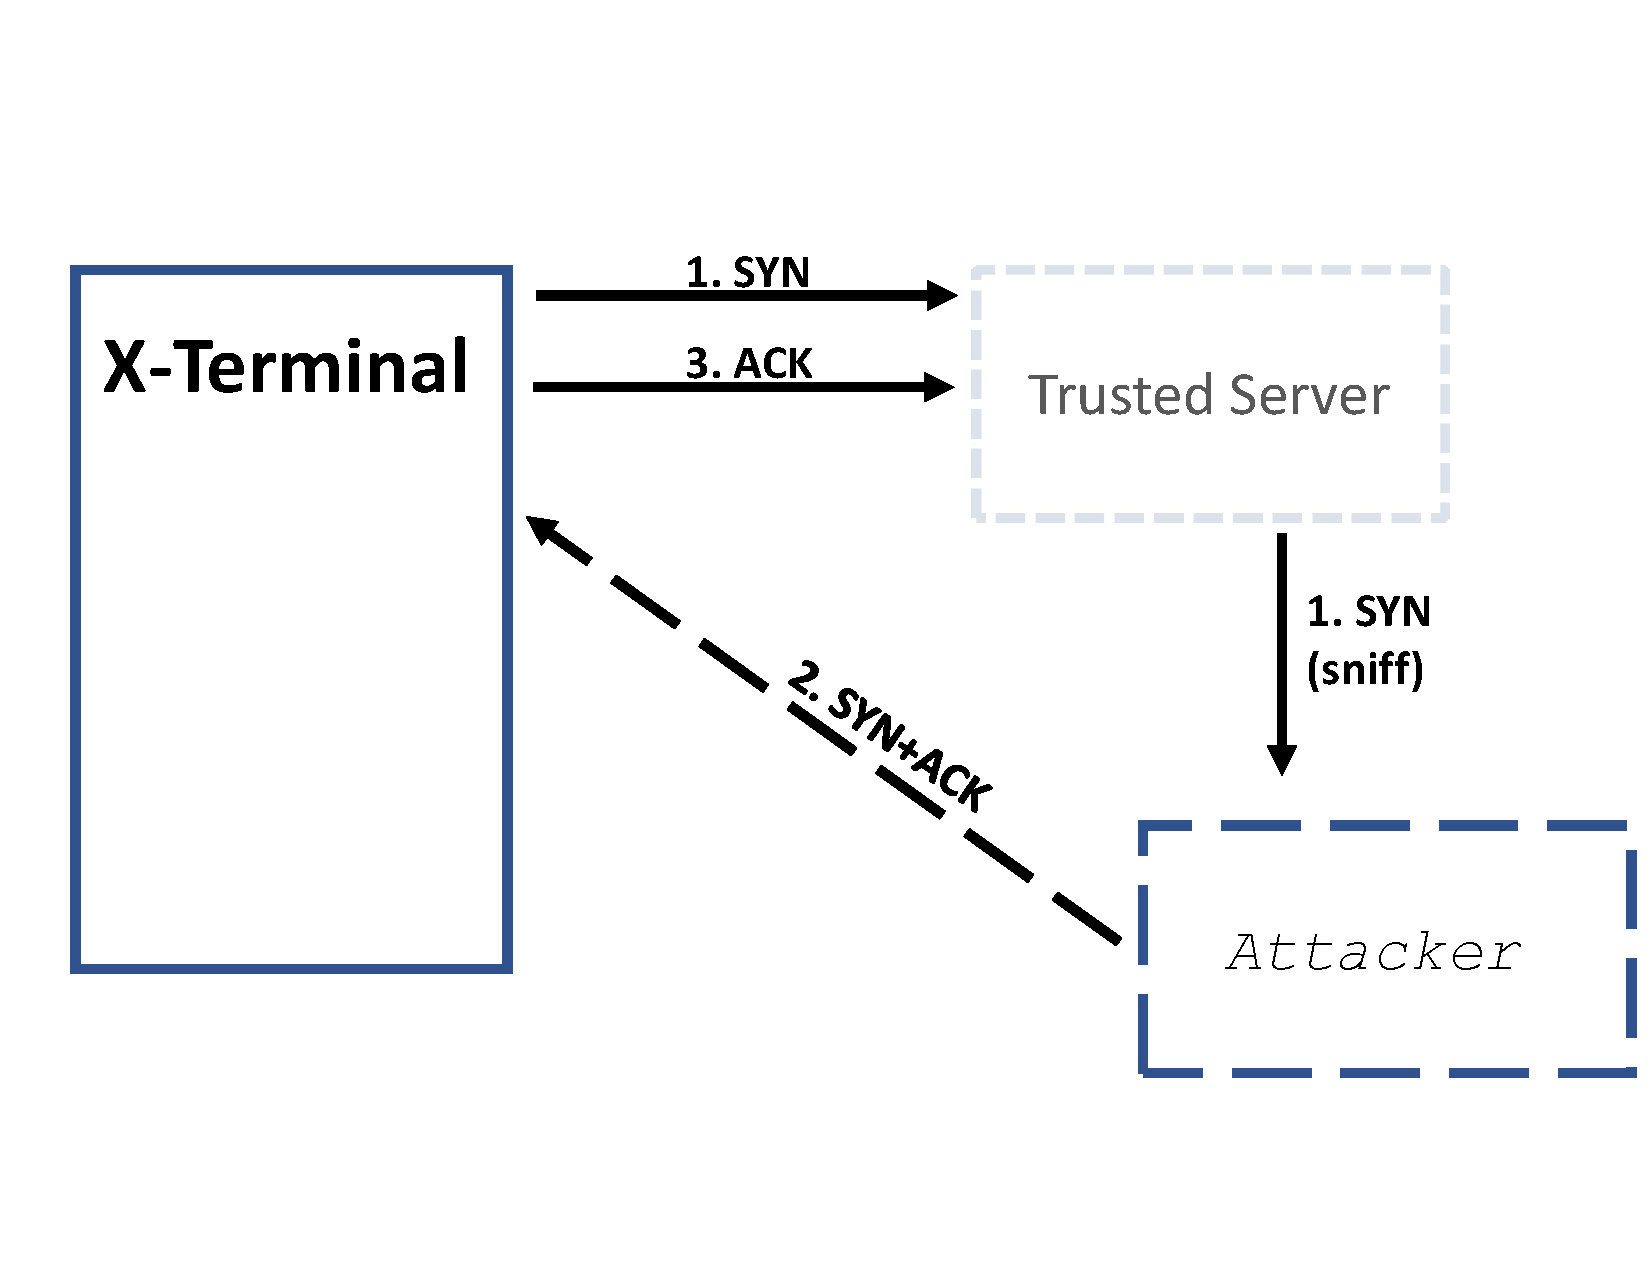
\includegraphics[width=0.6\textwidth]{\mitnickFigs/mitnick-diagram-2.pdf}
\caption{Second Connection}
\label{fig:second-conn}
\end{figure}


After the first connection has been established, X-Terminal will initiate 
the second connection. This connection is used by \texttt{rshd} to send 
out error messages. In our attack, we will not use this connection, but
if this connection is not established, \texttt{rshd} will stop without 
executing our command. Therefore, we need to use spoofing 
to help X-Terminal and the trusted server finish establishing this connection. 
See Figure~\ref{fig:second-conn}. 


Students need to write another sniff-and-spoof program, which
sniffs the TCP traffic going to the port 9090 of the trusted server (assuming
\texttt{9090} is used in Task 2.1). When it sees a SYN packet,
it should respond with a SYN+ACK packet. See Packet 7 
in Listing~\ref{listing:rsh} for an example.

If both connections have been successfully established, \texttt{rshd} 
will execute the command contained in the \rsh data packet. Please 
check the \texttt{/tmp} folder and see whether \texttt{/tmp/xyz} is created
and whether its timestamp matches the present time. Please 
include your evidence in your report. 



% *******************************************
% SECTION
% ******************************************* 
\section{Task 3: Set Up a Backdoor}

In Task 2, we only run a \texttt{touch} command in the attack to prove that we can
successfully run a command on X-Terminal. If we want to run
more commands later, we can always launch the same attack. That is quite inconvenient. 

Mitnick did plan to come back to X-Terminal. Instead of launching the attack
again and again, he planted a backdoor in X-Terminal after his initial attack. 
This backdoor allowed him to log into X-Terminal normally anytime he wanted, without 
typing any password. 
To achieve this goal, as we have discussed in 
Section~\ref{subsec:configuration}, 
all we need to do is to add the string \texttt{"+ +"} to
the \texttt{.rhosts} file (in a single line). We can
include the following command in our \rsh data.

\begin{lstlisting}
echo + + > .rhosts
\end{lstlisting}

Students should replace the \rsh command in Task 2 with
the \texttt{echo} command above, and then repeat the attack.   
If the attack succeeds, the attacker should be able to 
remotely log into X-Terminal using the following command,
and no password is needed: 

\begin{lstlisting}
$ rsh [X-Terminal's IP]
\end{lstlisting}



% *******************************************
% SECTION
% ******************************************* 
\section{Submission}

\seedsubmission



\end{document}



